% Chapter 3

\chapter{Transferencia de aprendizaje} % Main chapter title

\label{Chapter3} % For referencing the chapter elsewhere, use \ref{Chapter1} 

Un concepto esencial para este trabajo y para toda el área de aprendizaje profundo es la capacidad de transferir aprendizaje adquirido previamente de un problema poco acotado y poder lograr aprovechar este aprendizaje en problemas más acotados permitiendo así que las demandas de recursos como datos y tiempo de ejecución tengan más holgura.

\section{Concepto de transferencia}

Las redes neuronales capturan información en sus diferentes capas, sin embargo el hecho de que distintas capas aprenden cosas diferentes y la forma en que difieren permite transferir conocimiento a través de redes entrenadas para diferentes tareas. En las primeras capas se aprende información bastante abstracta con respecto a la tarea y conforme se avanza en la profundidad de la red se vuelve más específica la inforamción que se va aprendiendo.

\begin{figure}
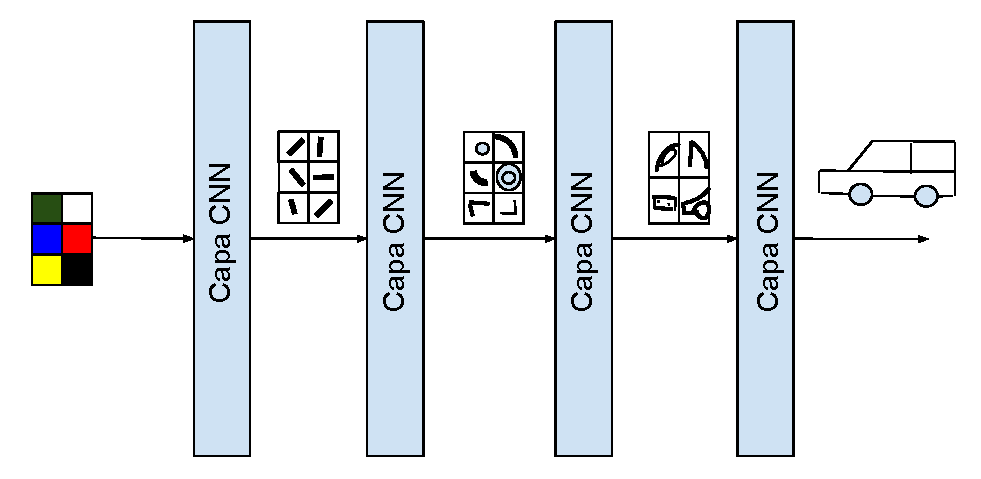
\includegraphics[scale=1]{Figures/learnbylayer.pdf}
\caption{Ejemplo ilustrativo de lo que podría aprender una red profunda de visión artificial para la detección de vehículos.}
\label{fig:learnbylayer}
\end{figure}

\textbf{Ejemplo ilustrativo.} En una red neuronal cuya tarea es en el área de visión artificial las primeras capas comienzan a entender conceptos de orillas horizontales o verticales; las siguientes capas podrán entender qué son esquinas circunferencias; las siguientes capas podrán entender límites de objetos; etc.

La información en las primeras capas de una red neuronal de visión artificial puede llegar a ser muy útil sin importar la tarea final o qué tan acotada esté. Por esta razón es posible tomar un modelo preentrenado en una tarea general, remover su capa final --- la cual determina el resultado final de esa tarea en específico --- y continuar con el proceso de entrenamiento con datos de la tarea más acotada y permitir que las nuevas capas no entrenadas aprovechen los conceptos de las capas anteriores para poder ellas tener le poder de predecir usando esa información los resultados correctos.



\section{Aplicación en otras áreas}
%Incluir trabajos relacionados
Para tener el contexto acerca de este concepto crucial para este trabajo debemos explorar otras áreas del aprendizaje profundo, en particular el área de visión artificial (computer vision en inglés). Este campo fue el que llevó a la explosión del aprendizaje profundo en el 2012 cuando una red denominada AlexNet dominó la competencia de ImageNet.

\textbf{ImageNet.} Este proyecto es una colección masiva de imágenes que están debidamente etiquetadas con cuadros encerrando los objetos detectados en una imagen. Debido a la cantidad exagerada de categorías y objetos encontrados en las imágenes y también la cantidad en sí de imágenes, se organiza un concurso de software todos los años para determinar cuál modelo es el mejor en visión artificial. Cuando en el 2012 una red de aprendizaje profundo ganó el concurso se generó motivación en explorar este campo más a fondo.

Esta tarea llegó a ser el estándar para poder determinar si un modelo podía \emph{ver} a nivel general. ¿Qué significa esto? La tarea de ver es una tarea muy basta y bastante general. Hay muchas características por considerar lo cual aumenta la complejidad de este problema.

% incluir ilustracion de imagenet aca

En CV existen muchas más tareas más acotadas que ver. Para estas sería muy útil poder utilizar información previamente aprendida con la finalidad no necesitar muchos datos para la tarea más específica. Por su misma naturlaza tendrá menos datos de entrenamiento.

\section{Aplicación en NLP}

\subsection{ULMFiT}